%!TEX encoding = UTF-8 Unicode

%!TEX root = ../compendium.tex

\Teamlab{\LabWeekSEVEN}

\begin{Goals}
%!TEX encoding = UTF-8 Unicode

%!TEX root = ../compendium.tex

\item Kunna skapa och använda arvshierarkier och förstå dynamisk bindning.
\item Kunna skapa använda en trait som bastyp i en arvshierarki.

\end{Goals}

\begin{Preparations}
\item Gör övning {\tt \ExeWeekSEVEN} i kapitel \ref{exe:W07}.
\item Läs på om och förstå arv
%!TEX encoding = UTF-8 Unicode
%!TEX root = compendium.tex
\item 
Diskutera i din samarbetsgrupp hur ni ska dela upp koden mellan er i flera olika delar, som ni kan arbeta med var för sig. En sådan del kan vara en klass, en trait, ett objekt, ett paket, eller en funktion. 
\item
Varje del ska ha en \emph{huvudansvarig} individ. 
\item
Arbetsfördelningen ska vara någorlunda jämnt fördelad mellan gruppmedlemmarna.
\item
När ni redovisar er lösning ska ni börja med att redogöra för handledaren hur ni delat upp koden och vem som är huvudansvarig för vad. 
\item
Den som är huvudansvarig för en viss del redovisar den delen.
\item 
Grupplaborationer görs i huvudsak som hemuppgift. Salstiden används primärt för redovisning.
\end{Preparations}

\subsection{Bakgrund}
I labben kommer sköldpaddor, \code{Turtle}, att få tävla mot varandra i ett lopp. Racet kommer att köras i ett \code{RaceWindow} som ärver från \code{SimpleWindow}. Först kommer en \code{RaceTurtle} att skapas, som ärver från \code{Turtle} och sedan kommer sköldpaddor med olika egenskaper att skapas. Dessa sköldpaddor kommer sedan att tävla i en turnering med 32 sköldpaddor. Det kommer att vara åtta sköldpaddor i varje deltävling och turneringen kommer att bestå av fyra kvartsfinaler, två semifinaler och tillsist en final.

\subsection{Obligatoriska uppgifter}

\Task \code{ColorTurtle}.

\Subtask Högerklicka på projektet \code{w07_turtlerace_team} och välj \code{Build Path} $\rightarrow$ \code{Configure Build Path}. Välj fliken \code{Projects} och tryck \code{Add...}. Markera projektet \code{w06_turtlegraphics} och tryck \code{OK}.

\Subtask Skapa en ny klass \code{ColorTurtle} som ärver från \code{Turtle} och tar in en extra parameter \code{color} av typen \code{java.awt.Color}. \code{Turtle} måste importeras från paketet \code{turtlegraphics}.

\Subtask Använd \code{override} på metoden \code{forward}, där färgen i \code{SimpleWindow} sparas undan och sedan ändras till den angivna färgen \code{color}. Anropa sedan metoden \code{forward} i \code{Turtle} och byt tillbaka färgen i \code{SimpleWindow} till den färg som sparades undan.

\Task \code{RaceWindow}

\Subtask Skapa \code{RaceWindow} som ärver från \code{SimpleWindow} med fix storlek och förbestämd titel. Lämplig storlek är 800x400. Det ska finnas två attribut \code{startX} och \code{endX} som är förbestämda och motsvarar start och mål.

\Subtask Skapa tre metoder \code{startX}, \code{endX} och \code{startY}. \code{startX} och \code{endX} ska returnera värdet på motsvarande attribut. \code{startY} ska ta in ett heltal \code{nbr} som är ett startnummer och returnera y-värdet för det startnumret. \code{startX} och \code{endX} är x-värdet för start- resp. mållinjen och \code{startY} är y-värdet för varje sköldpaddas startposition på startlinjen.

\Subtask Skapa en metod \code{draw} som ritar upp ett race i fönstret och skriver ut startnummer. Definiera gärna en klass som ritar upp ett start-/målfält. Bilden är enbart ett exempel på vad man kan göra. Rita något kul! Titeln och alla tävlande turtles kommer att skrivas ut senare i uppgiften.

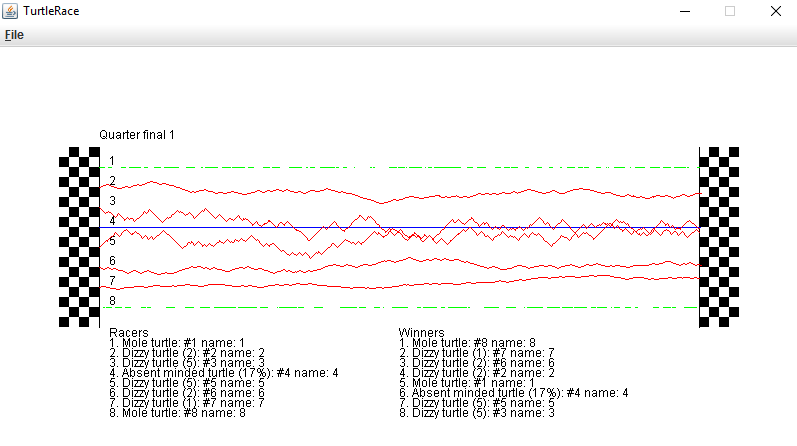
\includegraphics[width=\textwidth]{../img/turtlerace/RaceWindow}

\Subtask Skapa en metod \code{printTitle} som tar in en sträng och skriver ut den som titel på racet. Denna sträng skiljer sig från SimpleWindow-konstruktorns titelsträng, och används för att inuti fönstret skriva ut titeln för det nuvarande racet. Titelsträngen i SimpleWindow anger istället titeln för hela fönstret.

\begin{Code}
class RaceTurtle(private val w: RaceWindow,
var nbr: Int, val name: String) {
/**
* Takes one step of a random length 1 to 5
*/
def raceStep(): Unit = ???

/**
* Restarts the turtle at the finish line.
* To be used before each race
*/
def restart: Unit = ???

override def toString: String = ???
}
\end{Code}

\Task \code{RaceTurtle}.

\Subtask Implementera klassen \code{RaceTurtle} som ska ärva från \code{Turtle}. \code{Turtle} och \code{Point} behöver importeras från \code{turtlegraphics}. Startpositionen för en \code{RaceTurtle} hämtas från \code{RaceWindow}.\\Exempel på import-sats: \code{import turtlegraphics.Turtle}.

\Subtask Skapa en metod \code{printRacers} i \code{RaceWindow} som tar in en lista med \code{RaceTurtle}, ett $x$-värde för placering av utskriften i x-led, samt en titel på listan. Därefter skrivs listan ut vid angiven $x$-position och vid lämplig y-position. Se exemplet med listan \textit{Racers} och \textit{Winners}.

\Subtask Det går nu att testa \code{RaceTurtle} (för det krävs \code{TurtleRace}).

\Subtask Ändra så att \code{RaceTurtle} istället ärver från \code{ColoTurtle}. \code{RaceTurtle} behöver då ta in en parameter av typen \code{Color}.

\Task \code{TurtleRace}

\Subtask Implementera metoden \code{race} som ska börja med att skriva ut tävlande och titel i \code{RaceWindow}. Skapa en tom \code{ArrayBuffer} med namnet \code{winners} (för detta behöver man importera \code{scala.collection.mutable.ArrayBuffer}). Låt varje \code{RaceTurtle} ta ett steg tills en passerar mållinjen. Lägg över alla som passerat mållinjen i \code{winners} och kör detta tills alla \code{RaceTurtle} har hamnat i \code{winners}. Använd \code{SimpleWindow.delay(5)} mellan varje steg för att se animeringen. Skriv ut vinnarna i \code{RaceWindow} och vänta på musklick. Returnera listan med vinnare.

\Subtask Testa att köra ett race mellan åtta sköldpaddor.

\Task \code{Dizziness}, \code{AbsentMindness} och \code{Mole}

\Subtask Implementera tre \code{trait} som ärver från \code{RaceTurtle} och som \code{override} \code{raceStep} och \code{toString}. \code{toString} ska utöver \code{toString} från \code{RaceTurtle} även bestå av vilken typ av \code{RaceTurtle} det är och graden av yrsel/tankspriddhet den har.

\begin{itemize}

\item \code{Dizziness}. Slumpa ett heltal \code{dizziness} mellan 1 och 5. För varje steg ska en riktningsförändring slumpas fram som blir större desto större \code{dizziness} är. Slumpa även om den avviker åt höger eller vänster och använd \code{turnRight} och \code{turnLeft}.

\item \code{AbsentMindness}. Slumpa ett heltal \code{absent} mellan 0 och 99 som anger i procent hur tankspridd \code{RaceTurtle} är. För varje steg ska det vara \code{absent}\% chans att ett steg inte tas.

\item \code{Mole}. Med 50\% sannolikhet ska denna typ \code{RaceTurtle} gräva ner sig i marken. För varje steg ska det vara 50\% chans att pennan är uppe och 50\% chans att pennan är nere. Använd metoderna \code{penUp} och \code{penDown}.

\end{itemize}

\Task \code{TurtleTournament}

\Subtask Börja med att skapa en hjälpmetod \code{randTurtle} som tar in ett \code{RaceWindow}, ett nummer och ett namn som parameter. Slumpa med lika stor sannolikhet mellan att skapa en \code{ColorTurtle} med en av de tre olika egenskaperna och låt de olika egenskaperna ha olika färger.

\Subtask Skapa ett \code{RaceWindow}. Slumpa fram 32 sköldpaddor och låt åtta av dem tävla åt gången, i totalt fyra st  \code{TurtleRace} . Ta vara på vinnarna och låt de fyra bästa från varje lopp köra två lopp till. De fyra bästa från båda dessa loppen går vidare till finalen. \textbf{Tänk på att rensa \code{RaceWindow} efter varje lopp och rita ut det på nytt innan varje lopp}.

